\lecture{2}{24/1}

\begin{definition}[GPU]
    A \textbf{graphics processing unit} (GPU) is a processing unit designed
    for highly parallel operations.
\end{definition}

Thisis in contrast to a CPU which is designed to executed serially.
GPUs will split operations into a number of smaller operations which can
executed in parallel, and passes this suboperation to a \emph{cluster}
to execute it.

\begin{definition}[Graphics processor]
    A \textbf{graphics processor} accepts graphics commands from the CPU
    and executes it.
\end{definition}

Graphics commands are very simple and generic.
it draws the rendered result into the \emph{frame buffer}.

A graphics processor has separate 2D and 3D graphics commajnds, both
are based on Cartesian coordinates.

\begin{definition}[Frame buffer]
    A \textbf{frame buffer} is a memory space that stores a grid.
\end{definition}

Each grid cell stores a colour value / intensity.

In practise, we use a frame buffer to store an image as it is being rendered
or while it is being drawn by a display (or both).

\begin{definition}[Double buffering]
    \textbf{Double buffering} is a technique in which use two frame buffers
    to render images:
    \begin{enumerate}
        \item one is used for the image / frame that is currently being
        rendered; and
        \item the other one is used for the image / frame that is currently
        being displayed.
    \end{enumerate}
\end{definition}

\begin{example}[Examples of graphics modelling and programming tools]
    \hfill
    \begin{enumerate}
        \item Programs such as \emph{Blender} and \emph{Maga} are
        used for modelling;
        \item programs such as \emph{Photoshop} and \emph{Gimp} are
        used for image processing; and
        \item \emph{OpenGL}, \emph{WebGL}, \emph{DirectX}, \emph{Unity}, and
        \emph{Unreal} are examples of programming toolkits
        (typically used for games).
    \end{enumerate}
\end{example}

\chapter{GPU programming}

Let's revisit our definition of a GPU.

\begin{definition}[GPU v2]
    A \emph{GPU} is a specialised electronic circuit designed to
    rapidly manipulate and alter memory to accelerate the creation of
    images in a frame buffer intended for output to a display device.
\end{definition}

\begin{figure}
    \centering
    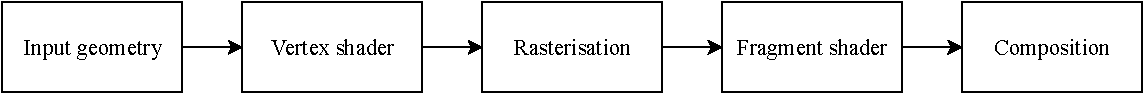
\includegraphics[width=\linewidth]{images/rendering-pipeline.pdf}
    \caption{A diagram of a simplified rendering pipeline.}
    \label{fig:rendering-pipeline}
\end{figure}

Figure \ref{fig:rendering-pipeline} shows a diagram of a simplified rendering
pipeline, we will look at each stage in this pipeline.

\begin{definition}[Vertex shader]
    A \textbf{vertex shader} is a program used in rendering that handles the
    processing of individual vertices.
\end{definition}

There should be a one-to-one mapping from all input to output vertices.

\begin{definition}[Rasterisation]
    \textbf{Rasterisation} is a process in rendering where vertices are
    converted to discrete objects called \textbf{fragments}.
\end{definition}

\begin{definition}[Fragment shader]
    A \textbf{fragment shader} is a progarm used in rendering that
    handles the processing of \emph{fragments}.
    It will process them into a set of colours and depth values.
\end{definition}
